% Auteur\,: Steve Prud’Homme
% Cette oeuvre, création, site ou texte est sous licence Creative Commons Attribution - Pas d’Utilisation Commerciale - Partage dans les Mêmes Conditions 4.0 International. Pour accéder à une copie de cette licence, merci de vous rendre à l'adresse suivante 
% http://creativecommons.org/licenses/by-nc-sa/4.0/ ou envoyez un courrier à 
% Creative Commons, 444 Castro Street, Suite 900, Mountain View, California, 94041, USA.

%\,:::SNIPET
%\,::: SECTION
% \section{Contexte} 
%		\begin{frame}[allowframebreaks]
%			\frametitle{}
%			\begin {itemize}
%				\item 
%			\end{itemize}
%		\end{frame}
%:::WATER MARK / FILIGRANE
%\usepackage{draftwatermark}
%\SetWatermarkLightness{0.5}
%\SetWatermarkAngle{25}
%\SetWatermarkScale{0.5}
%\SetWatermarkFontSize{2cm}
%\SetWatermarkText{Document de travail}

\documentclass[aspectratio=169]{beamer}
\usepackage{beamerthemesplit} % new 
\usepackage[french]{babel}
\usepackage[utf8]{inputenc}
\usepackage{tikz}
\usepackage[fixlanguage]{babelbib}
\selectbiblanguage{french}
% Natlib pour la bibliographie
\usepackage{natbib}
\usepackage{url}
\usetikzlibrary{mindmap,shadows,shapes,backgrounds}
\usepackage[T1]{fontenc}
\setbeamertemplate{bibliography item}[text]
\usepackage{multicol}
\def\firstcircle{(0,0) circle (1.5cm)}
\def\secondcircle{(60:2cm) circle (1.5cm)}
\def\thirdcircle{(0:2cm) circle (1.5cm)}
\definecolor{MightySlate}{RGB}{85,98,112}
\definecolor{Pacifica}{RGB}{78,205,196}
\definecolor{AppleChic}{RGB}{199,244,100}
\definecolor{CheeryPink}{RGB}{255,107,107}

\setbeamercolor{titlelike}{parent=structure}
\setbeamerfont*{title}{size=\huge}
\setbeamercolor{title}{bg=MightySlate, fg=white}
\setbeamercolor{author}{bg=Pacifica, fg=white}
\setbeamercolor{institute}{bg=AppleChic, fg=black}
\setbeamercolor{date}{bg=CheeryPink, fg=white}

\definecolor{DTUred}{RGB}{178,20,20}
\setbeamercolor*{palette primary}{use=structure,fg=white,bg=MightySlate}
\usepackage{helvet}
\begin{document}
\title{Plan d’action de conception et réalisation de projets de formation en ligne} 
\subtitle{Production}
\author{Steve Prud'Homme} 
\institute{Commission scolaire de Laval} 
\date{\today} 
	\usebackgroundtemplate{%
  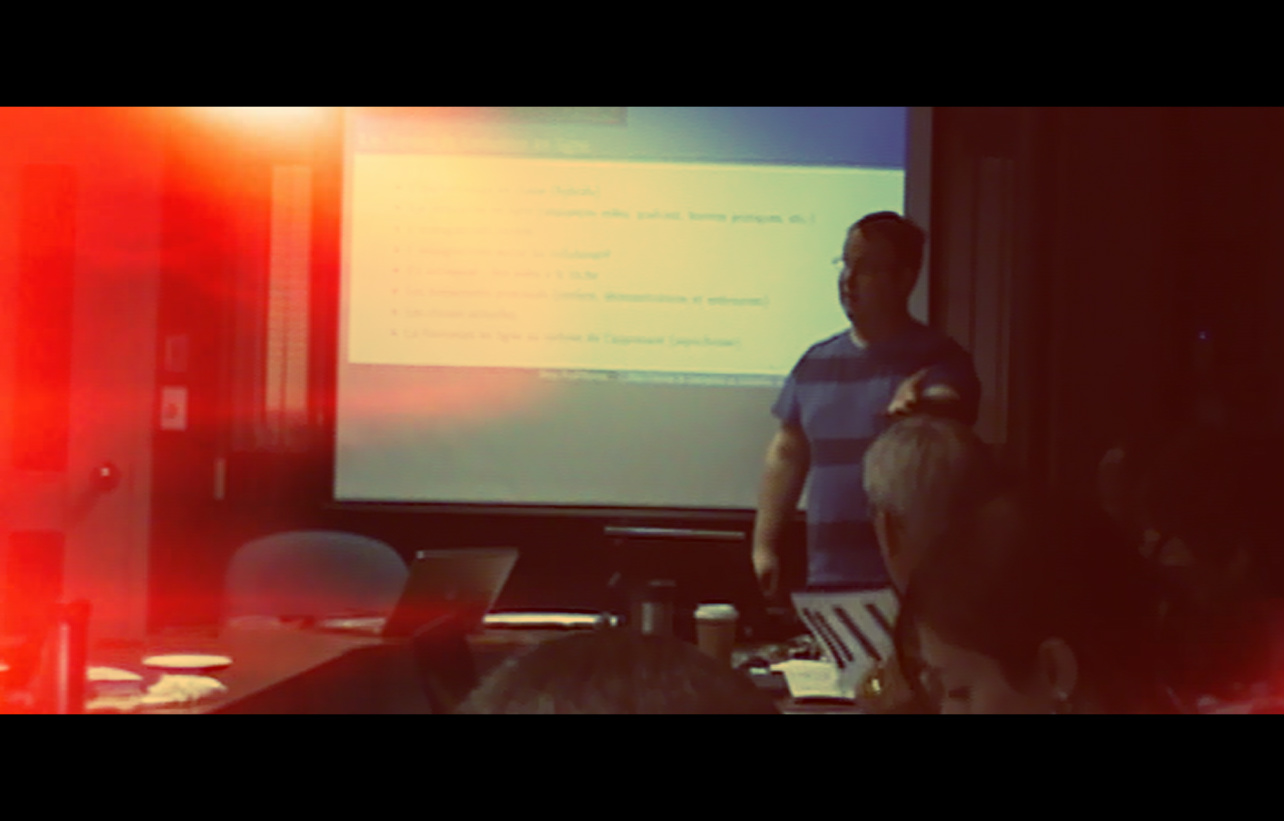
\includegraphics[width=\paperwidth]{back.jpg}} 

\begin{frame}

\end{frame}
\frame{\titlepage} 
\pagebreak
\usebackgroundtemplate{ } 
\frame[allowframebreaks]{\frametitle{Ordre du jour}\tableofcontents}


\section{Retour sur les étapes de production} 
\begin{frame}
\frametitle{Retour sur le flux de production}
\begin{figure}
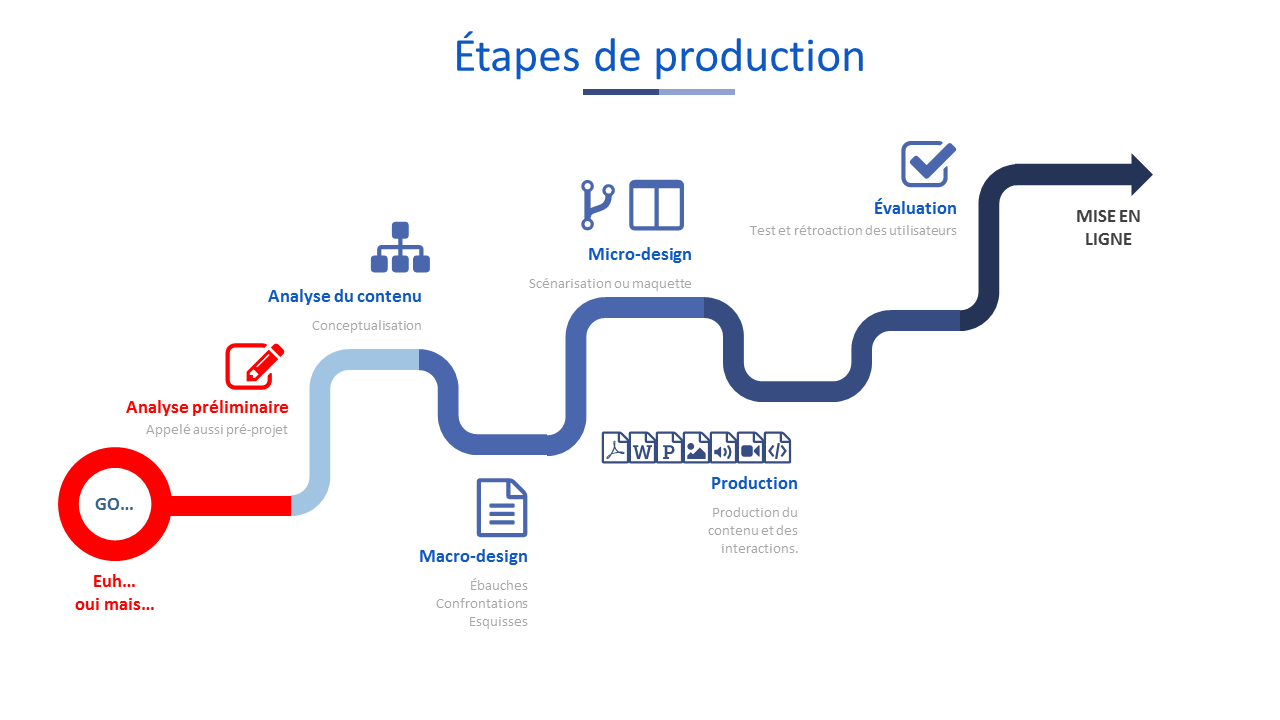
\includegraphics[scale=0.20]{flux.png}
\caption{Les applications générales du professionnel de l'éducation}
\end{figure}
\end{frame}


\section{Les formes de formation en ligne} 
\begin{frame}
\frametitle{Les formes de formation en ligne}
\begin{itemize}
\item L'apprentissage en classe (hybride)
\item Les ressources en ligne (séquences vidéo, podcast, bonnes pratiques, etc.)
\item L'enseignement mobile
\item L'enseignement social ou collaboratif 
\item En entreprise\,: des aides à la tâche
\item Les événements ponctuels (ateliers, démonstrations et webinaires)
\item Les classes virtuelles
\item La formation en ligne au rythme de l’apprenant (asynchrone)

\end{itemize}
\end{frame}


\section{Historique de l’écosystème de la formation en ligne} 
\subsection{Avant 2001 jusqu’à 2004}
\frame{\frametitle{Avant 2001 jusqu’à 2004\citep{clarey_organizational_2012}}
\begin{itemize}
\item Le catalogue de cours 
\item Le design pédagogique
\item Le matériel en ligne
\item L'environnement numérique d’apprentissage pour la formation en ligne

\end{itemize} 
}

\subsection{2001 à 2004}
\frame{\frametitle{2001 à 2004\citep{clarey_organizational_2012}}
\begin{itemize}
\item Le parcours d’apprentissage
\item Les rôles
\item L'interactivité
\item La simulation

\end{itemize} 
}


\subsection{2004 à 2007}
\frame{\frametitle{2004 à 2007\citep{clarey_organizational_2012}}
\begin{itemize}
\item L'apprentissage par compétences
\item Le \textit{Rapid E-learning} (information versus instruction)
\item L'apprentissage hybride (\textit{Blended learning}) 
\item Le développement d'environnements numériques d'apprentissage internes pour la formation des employés dans les entreprises 


\end{itemize} 
}

\subsection{2007 à 2011}
\frame{\frametitle{2007 à 2011\citep{clarey_organizational_2012}}
\begin{itemize}
\item Dans les entreprises, on parle de développement des carrières, de spécialisation pointue et de développement du leadership
\item La recherche, la collaboration, la communauté et l'architecture de l’information
\item L'apprentissage collaboratif et social, gestion du contenu et média riche
\item Les portails d’apprentissage, blogues, wikis, Twitter, mobilité et réseaux sociaux



\end{itemize} 
}

\subsection{2011 à aujourd'hui}
\frame{\frametitle{2011 à aujourd'hui\citep{clarey_organizational_2012}}
\begin{itemize}
\item L’internet mobile est partout
\item On localise les utilisateurs
\item Le flux d’information
\item En entreprise, l’apprentissage et la performance sont intégrés
\end{itemize} 
}



\section{L'écosystème de la formation en ligne} 
\subsection{Le schéma de l'écosystème de la formation en ligne}
\frame{\frametitle{Le schéma de l'écosystème de la formation en ligne}
\begin{figure}

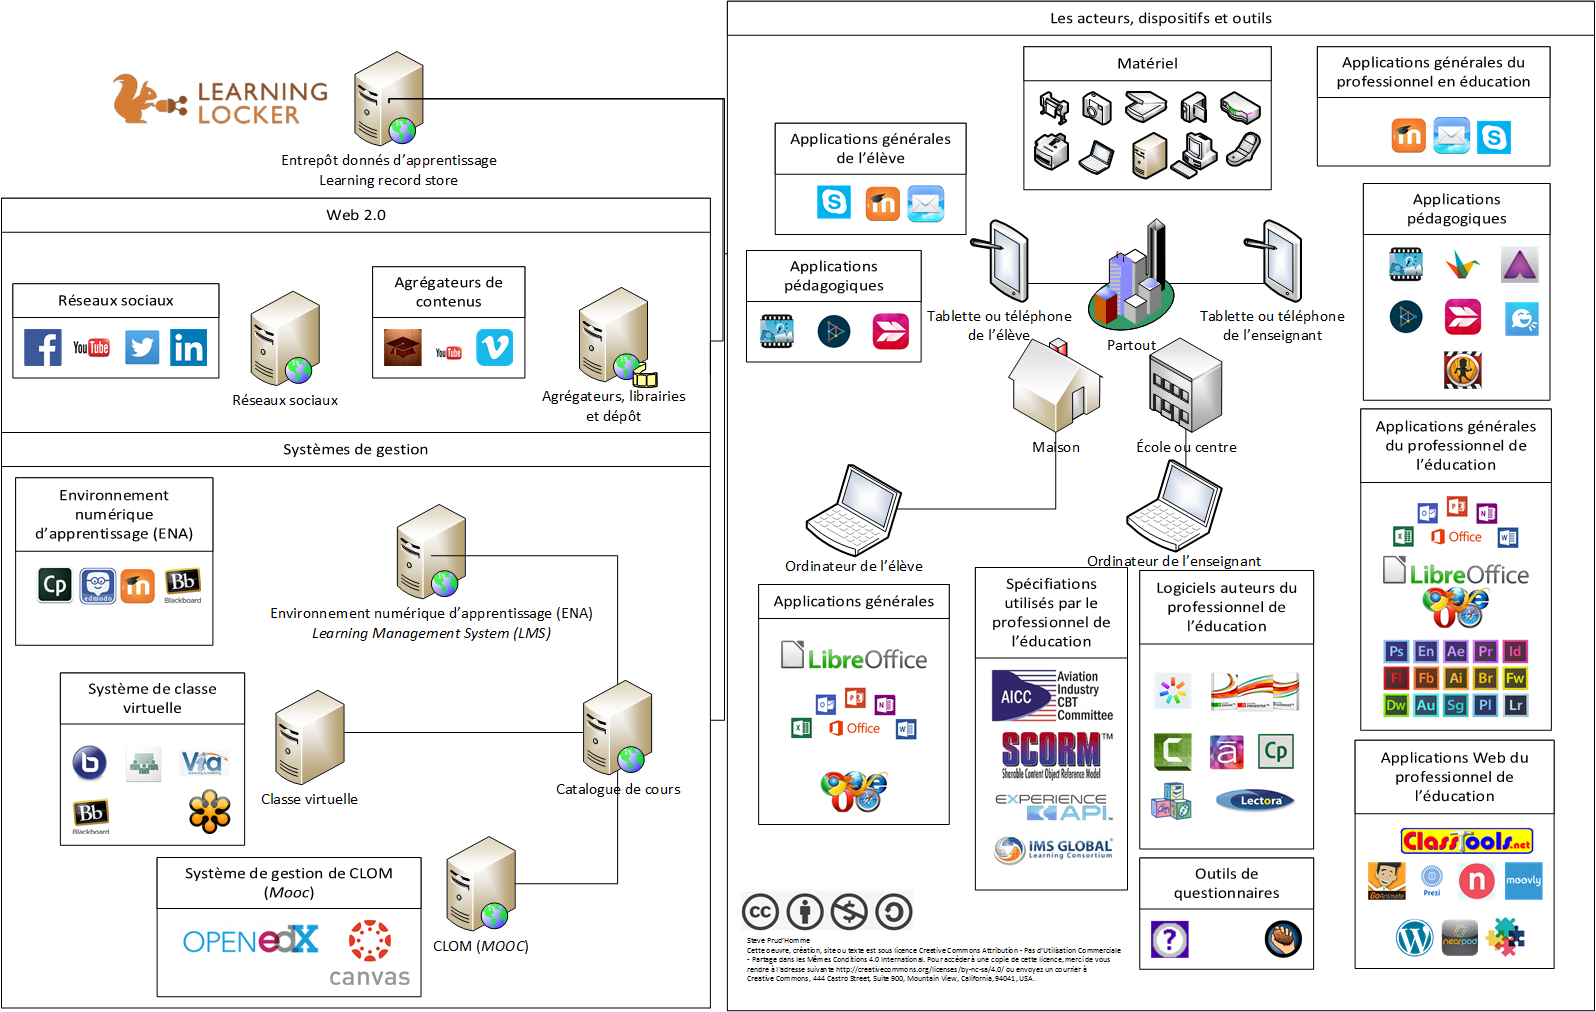
\includegraphics[scale=0.15]{ecosysteme.png}
\caption{Schéma de l'écosystème de la formation en ligne}
\end{figure}
}
\subsection{Les acteurs, outils et dispositifs}
\frame{\frametitle{Les acteurs, outils et dispositifs}
\begin{figure}

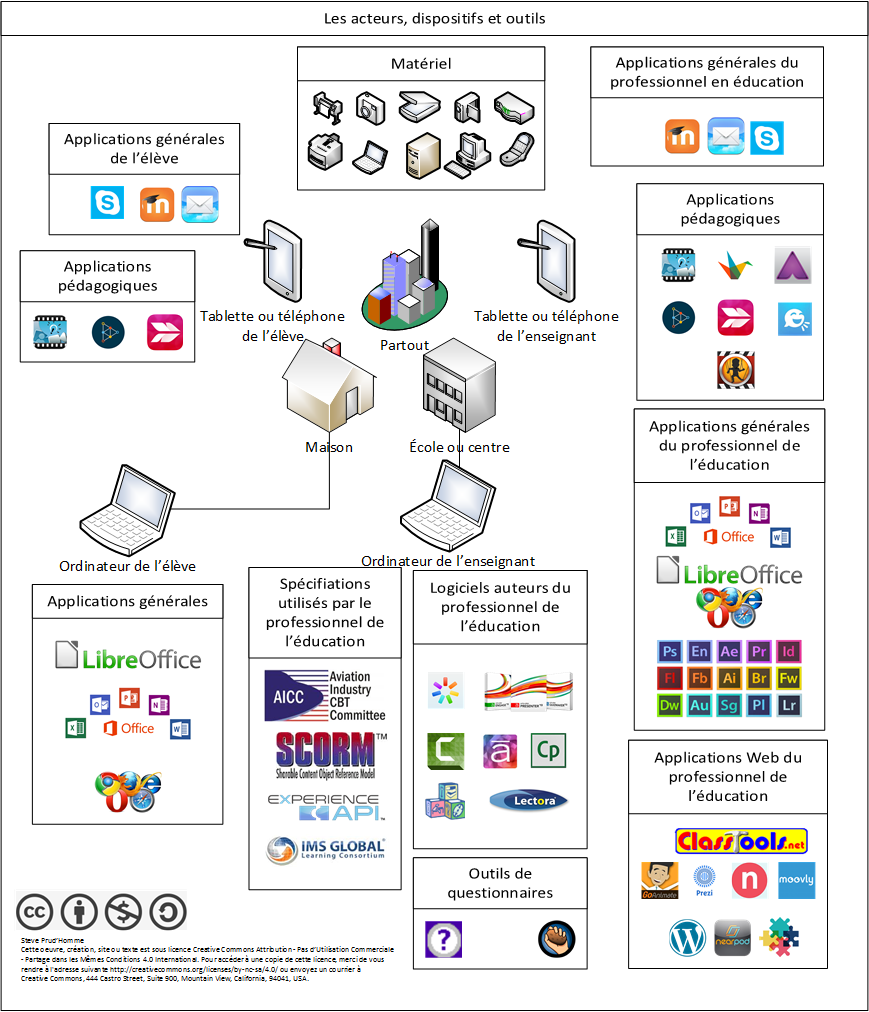
\includegraphics[scale=0.15]{acteurs.png}
\caption{Les acteurs, outils et dispositifs }
\end{figure}
}
\subsubsection{Le matériel}
\frame[allowframebreaks]{\frametitle{Le matériel}
\begin{figure}

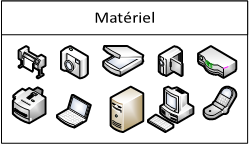
\includegraphics[scale=0.75]{materiel.png}
\caption{Le matériel }
\end{figure}
\begin{itemize}
\item Les serveurs
\item Les ordinateurs de bureau
\item Les ordinateurs portables
\item Les périphériques (caméras, scanneurs, imprimantes, etc.)
\item Le réseau filaire ou WiFi
\item Les dispositifs mobiles qui seront utilisés
\end{itemize} 
}
\subsubsection{Les applications générales du professionnel de l'éducation}
\frame[allowframebreaks]{\frametitle{Applications générales du professionnel de l'éducation}
\begin{figure}

\includegraphics[scale=0.35]{applicationgenerale.png}
\caption{Les applications générales du professionnel de l'éducation}
\end{figure}

\begin{itemize}
\item La suite Microsoft Office
\item La suite LibreOffice
\item Les navigateurs internet (Google Chrome, Mozilla Firefox, Microsoft Internet Explorer ou Edge, Opera et Safari)
\item La suite multimédia Adobe Creative Cloud (Photoshop, Illstrator, InDesign, Premiere, Aftereffect, Flash, DreamWeaver, etc.)
\end{itemize} 
}
\subsubsection{Les outils (logiciels) auteurs et chaînes éditoriales du professionnel de l'éducation}
\frame[allowframebreaks]{\frametitle{Les outils (logiciels)  auteurs et chaînes éditoriales du professionnel de l'éducation}
\begin{figure}

\includegraphics[scale=0.37]{logicielsauteur.png}
\caption{Les outils (logiciels) auteurs et chaînes éditoriales du professionnel de l'éducation}
\end{figure}
Programme informatique développé avec un langage auteur, qui permet de créer des applications sur mesure sans qu'il soit nécessaire de connaître la programmation. \citep{office_quebecois_de_la_langue_francaise_logiciel_2002}
\par 
Un logiciel auteur est un programme informatique utilisé pour associer différents médias. Il permet ainsi à l’auteur du contenu de créer une réalisation originale.
\par
Dans le domaine du e-learning, le logiciel auteur est l’outil qui permet de réaliser simplement et efficacement des formations interactives. \citep{e-doceo_definition_2016}
\par
\framebreak
\begin{itemize}
\item \href{https://www.ispringsolutions.com/ispring-free/}{iSprint (greffon de Microsoft PowerPoint)} 
\item \href{https://fr.articulate.com/products/presenter.php}{Articulate Presenter (greffon de Microsoft PowerPoint)}  
\item\href{https://fr.articulate.com/products/studio.php}{Articulate Studio}  
\item \href{http://www.adobe.com/ca_fr/products/captivate.html}{Adobe Captivate} 
\item \href{https://fr.articulate.com/products/storyline-why.php}{Articulate Storyline}
\item \href{http://trivantis.com/products/inspire-e-learning-software/}{Trivantis Lectora} 
\item \href{http://www.techsmith.fr/camtasia.html}{Camtasia}  
\item \href{http://scenari-platform.org/projects/opale/fr/pres/co/}{Scénari Opale\,: une chaîne éditoriale libre.}
\end{itemize} 
}
\subsubsection{Définir la chaîne éditoriale}
\frame {\frametitle{Définir la chaîne éditoriale}
\begin{figure}

\includegraphics[scale=0.5]{opale.png}
\caption{\href{http://scenari-platform.org/projects/opale/fr/pres/co/}{Scénari Opale\,: une chaîne éditoriale libre.}}
\end{figure}
Une chaîne éditoriale ou chaîne d'édition est le procédé industriel par lequel un document rédigé par un auteur est transformé en plusieurs déclinaisons publiables et publiées. Elle consiste à assister l'auteur dans le formatage de son document, à élaborer des modèles de documents, et à effectuer les conversions de fichiers nécessaires. Elle s'occupe également du stockage et de la diffusion des documents.
}
\subsubsection{Choisir un outil (logiciel) auteur\citep {pappas_christopher_11_2016}}
\frame[allowframebreaks]{\frametitle{Choisir un outil (logiciel) auteur \citep {pappas_christopher_11_2016}}
\begin{itemize}
\item Déterminer la facilité d'utilisation versus la souplesse
\item Considérer les compétences de l'équipe de développement
\item Déterminer quels sont vos objectifs
\item Garder toujours en tête l'apprenant
\item Déterminer si l'outil auteur supporte les modes de distribution désirés 
\item Déterminer si l'outil auteur supporte le niveau d'interactivité désiré 
\item Déterminer si l'outil auteur répond à vos besoins en matière de statistiques sur l'apprentissage ou la performance
\item Déterminer si l'outil auteur choisi est compatible avec les autres logiciels de formation en ligne que vous utilisez
\item Déterminer si vos livrables devront être supportés sur toutes les plateformes 
\item Déterminer si l'outil auteur dispose d'un bon système de questionnaire
\item Prendre le temps d'analyser toutes les options possibles
\end{itemize} 
}
\subsubsection{Outil auteur\,: liste de vérification}
\frame[allowframebreaks]{\frametitle{Outil auteur\,: liste de vérification\citep{mcintosh_elearning_2013}}
\begin{itemize}
\item S'assurer que l'interface est conviviale
\item Déterminer si la logique du logiciel est en lien avec celle du développeur
\item Faire un choix entre une application Web ou un logiciel sur l'ordinateur
\begin{itemize} 
\item  Déterminer le type de collaboration
\item  Déterminer le niveau de collaboration
\end{itemize} 
\item  Déterminer s'il existe un dépôt de ressources éducatives ou d'autres outils aidant la gestion du développement collaboratif
\begin{itemize} 
\item  Établir si l'outil auteur est compatible avec des outils de versionnage comme GIT, Mercurial, SVN (établir si le fichier natif est en mode texte pur ou binaire) 
\end{itemize} 
\item   Déterminer s'il est conforme au standard SCORM/AICC 
\item   Déterminer s'il est possible d'intégrer l'API Tin Can (xAPI) 
\item  Déterminer si l'outil permet de faire de la mise en page évoluée 
\begin{itemize} 
\item Déterminer s'il est possible de créer des gabarits 
\item Déterminer s'il y a déjà une banque de gabarits 
\item Déterminer s'il est possible de créer ses propres gabarits 
\item Déterminer si les feuilles de style sont supportées 
\end{itemize} 
\framebreak
\item Déterminer s'il est possible de publier dans une grande variété de formats 
\begin{itemize} 
\item HTML
\item XML
\item FLASH
\item HTML5
\item CD-ROM
\item EXÉCUTABLE
\item WORD / PDF
\end{itemize} 
\framebreak
\item Déterminer si les productions de cet outil auteur peuvent facilement être intégrées dans des scénarios de formation qui offrent des modalités de formation différentes 
\begin{itemize} 
\item  Cours en classe
\item  Laboratoire
\item  Classe virtuelle
\end{itemize} 
\item Déterminer si le logiciel auteur offre une banque de séquences vidéos, de sons, d'animations, d'avatars 
\begin{itemize} 
\item  Déterminer s'ils sont inclus dans le logiciel 
\item  Déterminer s'ils sont faciles d'utilisation 
\item  Établir quels sont les formats de ces fichiers et s'ils répondent à vos préférences, ou les standards utilisés 
\end{itemize} 
\item  Déterminer si l'outil offre la possibilité de faire des captures d'écran (image et vidéo) ainsi que des outils de simulation de logiciels 
\item Déterminer s'il est possible de créer autant des mises en situation réelles que des simulations de logiciels. 
\item Déterminer s'il est possible d'importer ou d'exporter d'autres outils auteurs 
\item Déterminer s'il est possible de modifier le thème graphique d'une capsule afin de l'adapter à la charte graphique (signature graphique) de l'organisation 
\framebreak
\item Déterminer si le logiciel auteur offre une navigation flexible pour les apprenants 
\begin{itemize} 
\item  Structure du cours
\item  Table des matières
\item  Glossaire
\item  Questions fréquentes
\item  Possibilité d'aller n'importe où dans le cours
\item  Recherche
\end{itemize} 
\item  Déterminer si l'apprenant peut lui-même personnaliser le thème de la capsule 
\item  Déterminer si vous contrôlez les parcours d'apprentissage ou s'ils sont libres 
\item  Déterminer s'il sera possible de générer des arborescences basées sur les choix des apprenants ou sur les résultats aux questionnaires
\item  Déterminer si les productions sont\,: \textit{adaptative}, c'est-à-dire que l'apprenant peut faire son parcours plus ou moins rapidement s'il obtient de bons résultats lors des questionnaires, ou par la remédiation s'il n'a pas de bons résultats
\item Déterminer s'il est possible et permis d'imprimer ou de sauvegarder les contenus d'une capsule interactive
\framebreak
\item Déterminer s'il y a de l'interactivité
\begin{itemize} 
\item Des questionnaires et questions
\item Des simulations
\item Des simulations de logiciels
\item Des jeux
\item Des interactions sociales
\item La possibilité de contacter quelqu'un s'il y a un problème
\item Des discussions de groupe
\item Des travaux pratiques
\end{itemize} 
\item Déterminer s'il y a des plugiciels ou modules complémentaires disponibles pour ce logiciel auteur afin d'avoir la possibilité d'ajouter des fonctionnalités
\item Déterminer s'il y a des plugiciels ou modules complémentaires disponibles pour ce logiciel auteur afin d'avoir la possibilité d'ajouter des fonctionnalités
\item Déterminer s'il est possible de consulter le contenu en étant hors-ligne
\item Déterminer s'il est possible de diviser le contenu en petits morceaux
\item Déterminer s'il est possible de consulter la formation sur des dispositifs mobiles 
\begin{itemize}
 \item Déterminer si le logiciel exporte en HTML 5
 \item Dimensionnement relatif des différents blocs de la page
\item  Utilisation des règles CSS différentes en fonction des caractéristiques du terminal de consultation. Le plus communément, il s'agit des règles appliquées en fonction de la largeur du terminal. Ces différentes largeurs sont appelées « \,points de rupture\,» et correspondent à un besoin de modifier la mise en page à partir d'un certain seuil critique pour la facilitation de la navigation et de la lecture du contenu.
\end{itemize} 
\end{itemize} 

}
\subsubsection{La triade HTML-CSS-JAVASCRIPT \citep {durant_html_2014}}
\frame{\frametitle{La triade HTML-CSS-JAVASCRIPT)\citep {durant_html_2014}}
\begin{multicols}{2}
\begin{tikzpicture}
    \begin{scope}[shift={(3cm,-5cm)}, fill opacity=0.5]
        \fill[red] \firstcircle;
        \fill[green] \secondcircle;
        \fill[blue] \thirdcircle;
        \draw \firstcircle node[below] {$CSS$};
        \draw \secondcircle node [above] {$HTML$};
        \draw \thirdcircle node [below] {$JAVASCRIPT$};
    \end{scope}
\end{tikzpicture}
\vfill
\columnbreak
\textbf {HTML}
\par Structure d'une page ou du contenu
\par Interactivité de base
\par \textbf {CSS}
\par Design de la page
\par L'aspect visuel
\par Interactivité simple
\par \textbf {Javascript}
\par Script de manipulation de la page
\par Interactivité de haut niveau

\end{multicols}

}
\subsubsection{Définir le versionnage (authoring software)\citep {office_quebecois_de_la_langue_francaise_logiciel_2002}}
\frame[allowframebreaks]{\frametitle{Définir le versionnage (\textit {authoring software})\citep {office_quebecois_de_la_langue_francaise_logiciel_2002}}
Mécanisme qui consiste à conserver la version d'une entité logicielle quelconque, de façon à pouvoir la retrouver facilement, même après l'apparition et la mise en place de versions plus récentes  
\par
Le versionnage peut s'appliquer, entre autres, à un logiciel, à un fichier, à un composant logiciel, à une page Web ou à un SGBD
\par
Il ne faut pas confondre le versionnage et la mise à jour. En effet, lors d'une mise à jour, on ne se préoccupe pas nécessairement de conserver les anciennes versions d'un logiciel.  
}
\subsubsection{Définir le SCORM (Sharable Content Object Reference Mode)\,?\citep {e-doceo_definition_2016}}
\frame[allowframebreaks]{\frametitle{Définir le SCORM (\textit {Sharable Content Object Reference Mode}) \citep {e-doceo_definition_2016}}
Il s’agit d’un modèle de référence de formation diffusé par Internet. La norme SCORM permet de certifier que les contenus produits respectent des standards prédéfinis garantissant des fonctionnalités évoluées dans le domaine de la formation \textit {e-learning} telles que la gestion du \textit {tracking} des apprenants.
\par
Cela permet de garantir l’interopérabilité.
\par
Actuellement, deux standards SCORM sont en service\,: le SCORM 1.2 (en fin de vie [compatible avec Moodle]) et le SCORM 2004.
}
\subsubsection{Définir le AICC (Aviation Industry CBT (Computer-Based Training) Committee)\,?\citep {e-doceo_definition_2016}}
\frame[allowframebreaks]{\frametitle{Définir lele AICC (\textit {Aviation Industry CBT (Computer-Based Training) Committee})\citep {e-doceo_definition_2016}}
Cette norme permet de garantir certaines spécificités\,: gestion du chargement d'un contenu dans un ENA, standardisation de la communication entre le contenu et le LMS, adaptation de la pédagogie du contenu en fonction de l'apprenant. Cela permet de garantir l’interopérabilité.

}
\subsubsection{Définir le Tin Can API (ou Experience API, ou encore xAPI)\,?\citep {theler_comprendre_2013}}
\frame[allowframebreaks]{\frametitle{Définir le  le Tin Can API (\textit {ou Experience API, ou encore xAPI}) \citep {theler_comprendre_2013}}

\begin{figure}


\includegraphics[scale=0.4]{tincan.png}
\caption{Logo Tin Can Api}
\end{figure}
\framebreak

Tin Can API (ou Experience API, ou encore xAPI, selon que l’on utilise le nom donné par ses auteurs ou par leurs mandants) est une norme récemment finalisée qui s’inscrit dans un dispositif destiné à remplacer SCORM. Comme sa prédécesseure, Tin Can API sert à suivre des activités de formation et à les transmettre à une plateforme de gestion de formation.
Pourquoi remplacer SCORM par Tin Can API\,?
\framebreak
\par Tin Can est né de la volonté d’ADL, déjà à l’origine de SCORM, de proposer une norme plus souple et adaptée à la multiplicité des «unités de formation» (comme SCORM 2.0 avait essayé de le faire auparavant). À l’inverse de SCORM, qui nécessite une plateforme LMS centralisant l’ensemble des contenus de formations, Tin Can étend la notion d’apprentissage à n’importe quels contenus, où qu’ils se trouvent et quelles que soient leur nature\,: une vidéo sur YouTube, un entretien avec un collègue, la réalisation d’une tâche ou encore la lecture d’un article de blog comme celui-ci. \par Avec Tin Can, c’est donc la définition du mot «apprentissage» qui est revue pour s’adapter aux façons modernes de consommer de la connaissance.

}

\subsubsection{Définir le HTML (HyperText Markup Language) \citep {office_quebecois_de_la_langue_francaise_langage_2002}}
\frame[allowframebreaks]{\frametitle{Définir le HTML  (\textit {HyperText Markup Language}) \citep {office_quebecois_de_la_langue_francaise_langage_2002}}

\begin{figure}

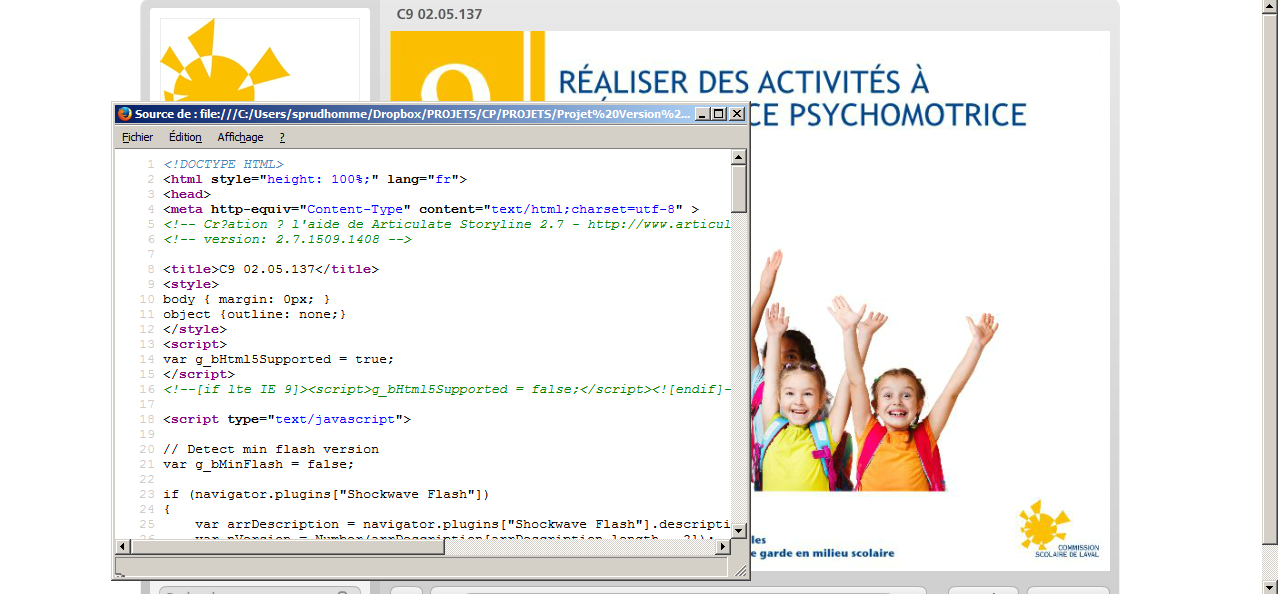
\includegraphics[scale=0.15]{html.png}
\caption{exemple de code HTML}
\end{figure}
Langage de balisage de texte qui permet la création de documents hypertextes affichables par un navigateur Web.  



}
\subsubsection{Définir le XML ou le langage de balisage extensible (HyperText Markup Language)\,? \citep{office_quebecois_de_la_langue_francaise_langage_2006}}
\frame[allowframebreaks]{\frametitle{Définir le XML ou le langage de balisage extensible (\textit {Extensible Markup Language})?\citep{office_quebecois_de_la_langue_francaise_langage_2006}}

\begin{figure}

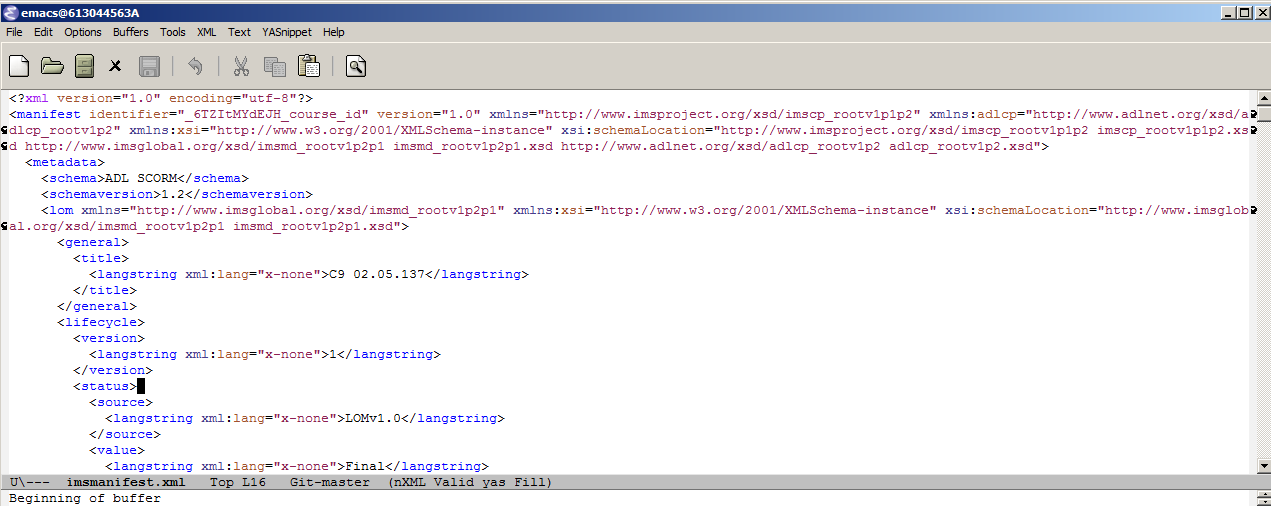
\includegraphics[scale=0.15]{xml.png}
\caption{exemple de code XML (Manifeste SCORM)}
\end{figure}
\par Langage de balisage [...], conçu pour faciliter la modification et la validation des programmes qui en découlent, et principalement utilisé pour l'échange de l'information entre des systèmes informatiques hétérogènes.
\par Créé au départ pour la diffusion de documents complexes et volumineux destinés au Web, le langage XML sert aujourd'hui surtout de norme d'échange pour une variété de données très étendues. C'est un métalangage qui permet de séparer le contenu d'un document de sa présentation et de définir son propre langage pour décrire ce contenu (OQLF, 2006).


}
\subsubsection{Choisir un outil de questionnaire\citep{mcintosh_elearning_2013}}
\frame[allowframebreaks]{\frametitle{Choisir un outil de questionnaire\citep{mcintosh_elearning_2013}}

\begin{figure}

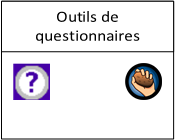
\includegraphics[scale=0.7]{questionnaire.png}
\caption{Logiciels de conception de questionnaires}
\end{figure}
\framebreak
Plusieurs logiciels auteurs contiennent des dispositifs de conception de questionnaires. Il y a aussi des logiciels spécialisés.

\begin{itemize} 
\item Déterminer s'il est possible de bâtir un questionnaire à partir d'une banque de questions.
\item Déterminer si les questions peuvent être réparties au hasard
\item Déterminer si les leurres peuvent être répartis au hasard
\item Déterminer s'il est possible de fixer le nombre d'essais
\item Déterminer s'il est possible de préciser une durée
\framebreak
\item Déterminer s'il est possible de créer plusieurs types de questions
\begin{itemize} 
\item Choix multiples
\item Choix unique
\item Transformation de phrase
\item Textes troués
\item Corrections d'erreurs
\item Vrais ou faux
\item Association
\item Échelle
\item Calculs mathématiques (avec entrées variables)
\item Réponse numérique
\item Réponse courte
\item Texte (avec correction de la réponse par l'enseignant)
\end{itemize} 

 \item Déterminer quel est le type de rétroaction possible
\begin{itemize} 
\item Déterminer s'il est possible d'appliquer un pointage sur tout le test
\item Déterminer s'il est possible de donner la réponse correcte après chaque question
\item Déterminer s'il est possible de commencer le questionnaire
\item Déterminer si le pointage est gardé à titre de statistiques


\end{itemize} 

\end{itemize} 


}

\subsubsection{Utiliser des applications Web pour créer du contenu}
\frame[allowframebreaks]{\frametitle{Utiliser des applications Web pour créer du contenu}

\begin{figure}


\includegraphics[scale=0.6]{webapp.png}
\caption{Applications Web}
\end{figure}
Voici des exemples d'applications qui peuvent être utilisées pour créer du contenu pour la formation en ligne. Attention\,: ces applications, lorsqu'elles sont payantes, ont souvent des modèles d'affaires basés sur l'abonnement. Il est souvent impossible de télécharger un fichier source.
\begin{itemize} 
\item \href{https://goanimate.com/}{GoAnimate} animation 2d
\item \href{http://www.nawmal.com/}{Nawmal}  
\item \href{http://www.nearpod.com/}{Nearpod}
 
\end{itemize} 
}
\subsubsection{Utiliser des applications iPad pour créer du contenu}
\frame[allowframebreaks]{\frametitle{Utiliser des applications iPad pour créer du contenu}

\begin{figure}

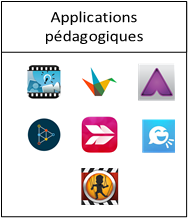
\includegraphics[scale=0.6]{ipad.png}
\caption{Applications iPad}
\end{figure}
Voici des exemples d'applications qui peuvent être utilisées pour créer du contenu pour la formation en ligne. Attention\,: ces applications, sont utilisées sur iPad et sont des applications bac de sable. Il est souvent difficile d'en extraire un fichier source.

}
\section{Systèmes de gestion} 
\begin{frame}
\frametitle{Systèmes de gestion}
\begin{figure}
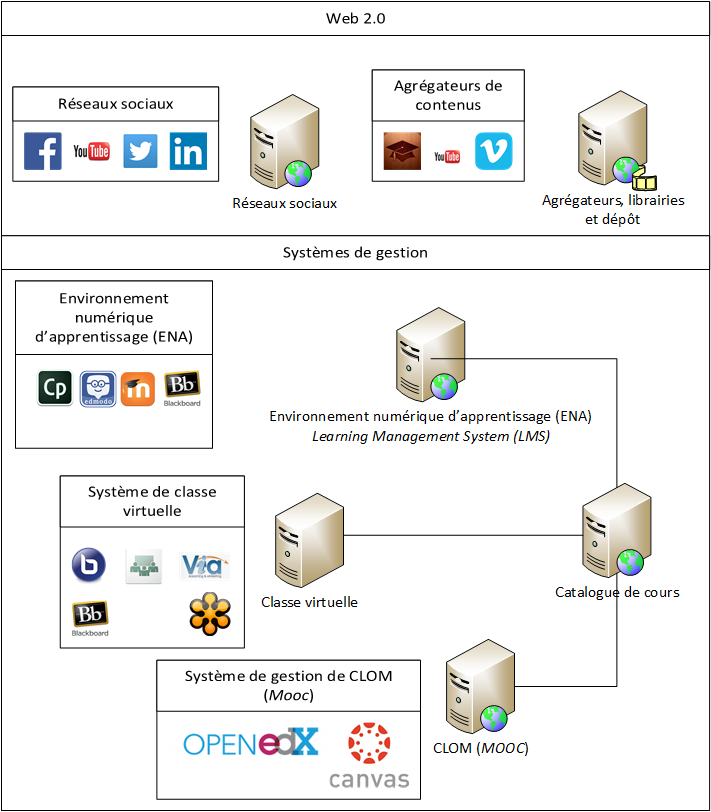
\includegraphics[scale=0.15]{systemegestion.png}
\caption{Les systèmes de gestion}
\end{figure}
\end{frame}
\section{Le Web 2.0} 
\begin{frame}
\frametitle{Le Web 2.0}
\begin{figure}
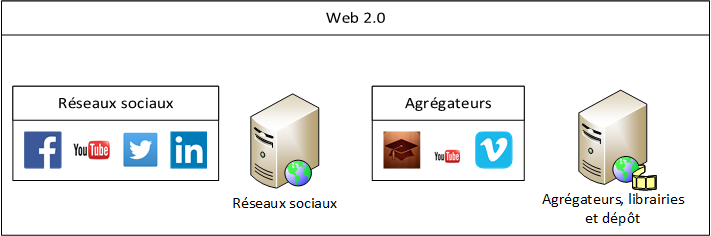
\includegraphics[scale=0.6]{web2.png}
\caption{Le Web 2.0}
\end{figure}
\end{frame}
\section{Le LRS (Learning Record Store)} 
\begin{frame}[allowframebreaks]
\frametitle{Le LRS (\textit{Learning Record Store})\citep{traore_learning_2015}}
\begin{figure}

\includegraphics[scale=0.75]{lrs.png}
\caption{Le LRS}
\end{figure}
\framebreak
\begin{itemize} 
\item Un élément nouveau et central de l'écosystème xAPI
\item Un entrepôt de stockage des énoncés (données) des différentes expériences d'apprentissage
\item Il peut résider à l'intérieur ou à l'extérieur d'un LMS
\item Il permet la génération de rapports et l'analyse des expériences d'apprentissage
\end{itemize} 
\end{frame}

%\section{Bibliographie}
%\subsection{Bibliographie}
%\frame[allowframebreaks]{\frametitle{Bibliographie}

\bibliographystyle{apalike}
\bibliography{bibliographie} %bibtex file name without .bib extension
%}
\end{document}

